\chapter{Преглед имплементираног система}

\begin{figure}[h!]
	\centering
	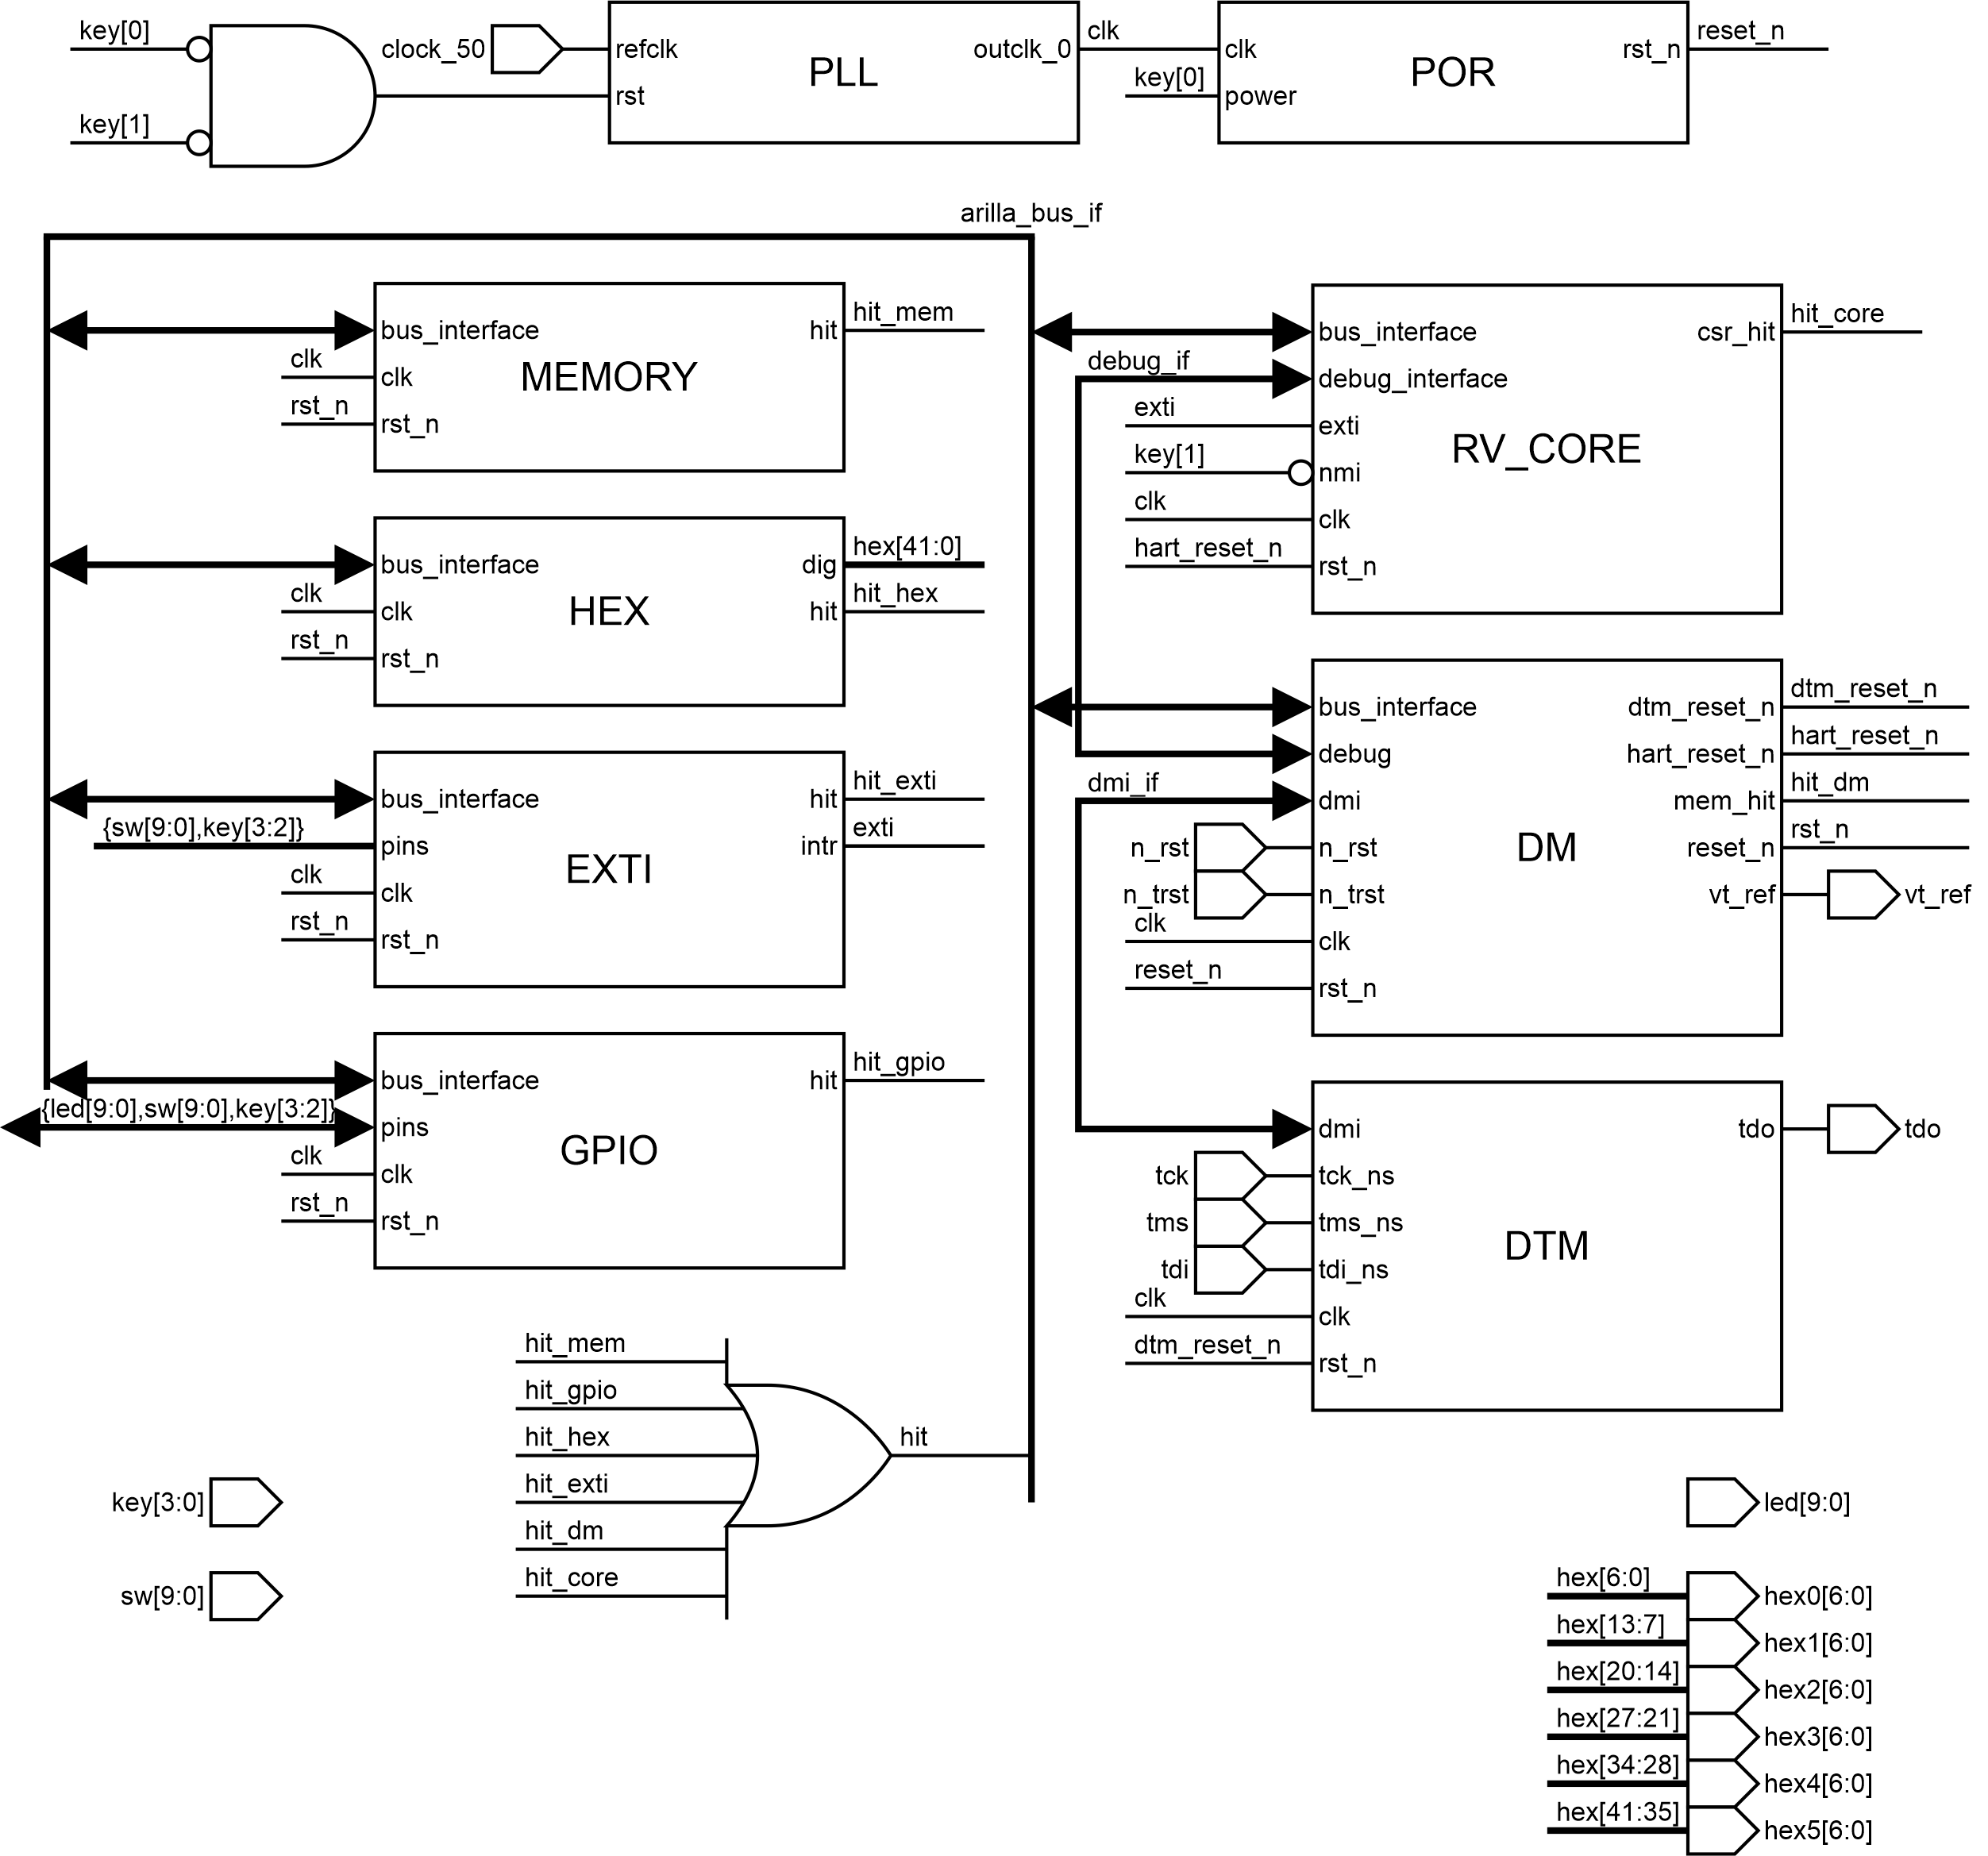
\includegraphics[width=\textwidth]{top}
	\caption{Дијаграм комплетног система}
	\label{fig:top}
\end{figure}

На слици \ref{fig:top} су приказане компоненте које сачињавају имплементирани систем, \рисцв{} језгро, \дм{} i \дтм{} су објашњени у својим поглављима, док су остале компоненте укратко објашњене у овом поглављу. Систем је дизајниран да буде конфигурабилан, што је постигнуто комбинацијом параметризованих компоненти и конфигурационих фајлова са дефиницијама макроа који садрже конкретне вредности параметара. Овај комбиновани приступ користи предности параметара (провера типова, инстанцирање исте компоненте са различитим вредностима параметара) а додатно сакупља све подесиве вредности на једно место. 

\lstinputlisting[language=Verilog, caption=Пример конфигурације система]{../src/system/system.svh}

Конфигурација система приказана изнад на почетку дефинише параметре самог језгра: ширину и број регистара, фиксне адресе на којима се налазе прекидне рутине за ресет и немаскирајући прекид, подразумевана вредност адресе прекидне рутине за остале прекиде и изузетке, подразумевану вредност бита који означава да ли су прекиди векторисани или не, ширину меморијске адресе и бајта у битима. Након тога је дефинисана меморијска мапа са базним адресама и величинама за меморију и периферије. На крају се налази конфигурација трајања ресет сигнала, ширина адресе \дми{} магистрале и базна адреса помоћних регистара за дебаговање.

\section{Сигнал такта и ресет система}

Слика \ref{fig:clkrst} приказује компоненте и сигнале који учествују у генерисању сигнала такта за остатак система и мрежи ресет сигнала. На слици су обележене фреквенције сигнала такта, као и описи мање очигледних сигнала. Сигнали са стрелицом која улази у компоненту или списак компоненти представља сигнал такта за те компоненте, док квадратић представља ресет сигнал те компоненте. 

\begin{figure}[h!]
	\centering
	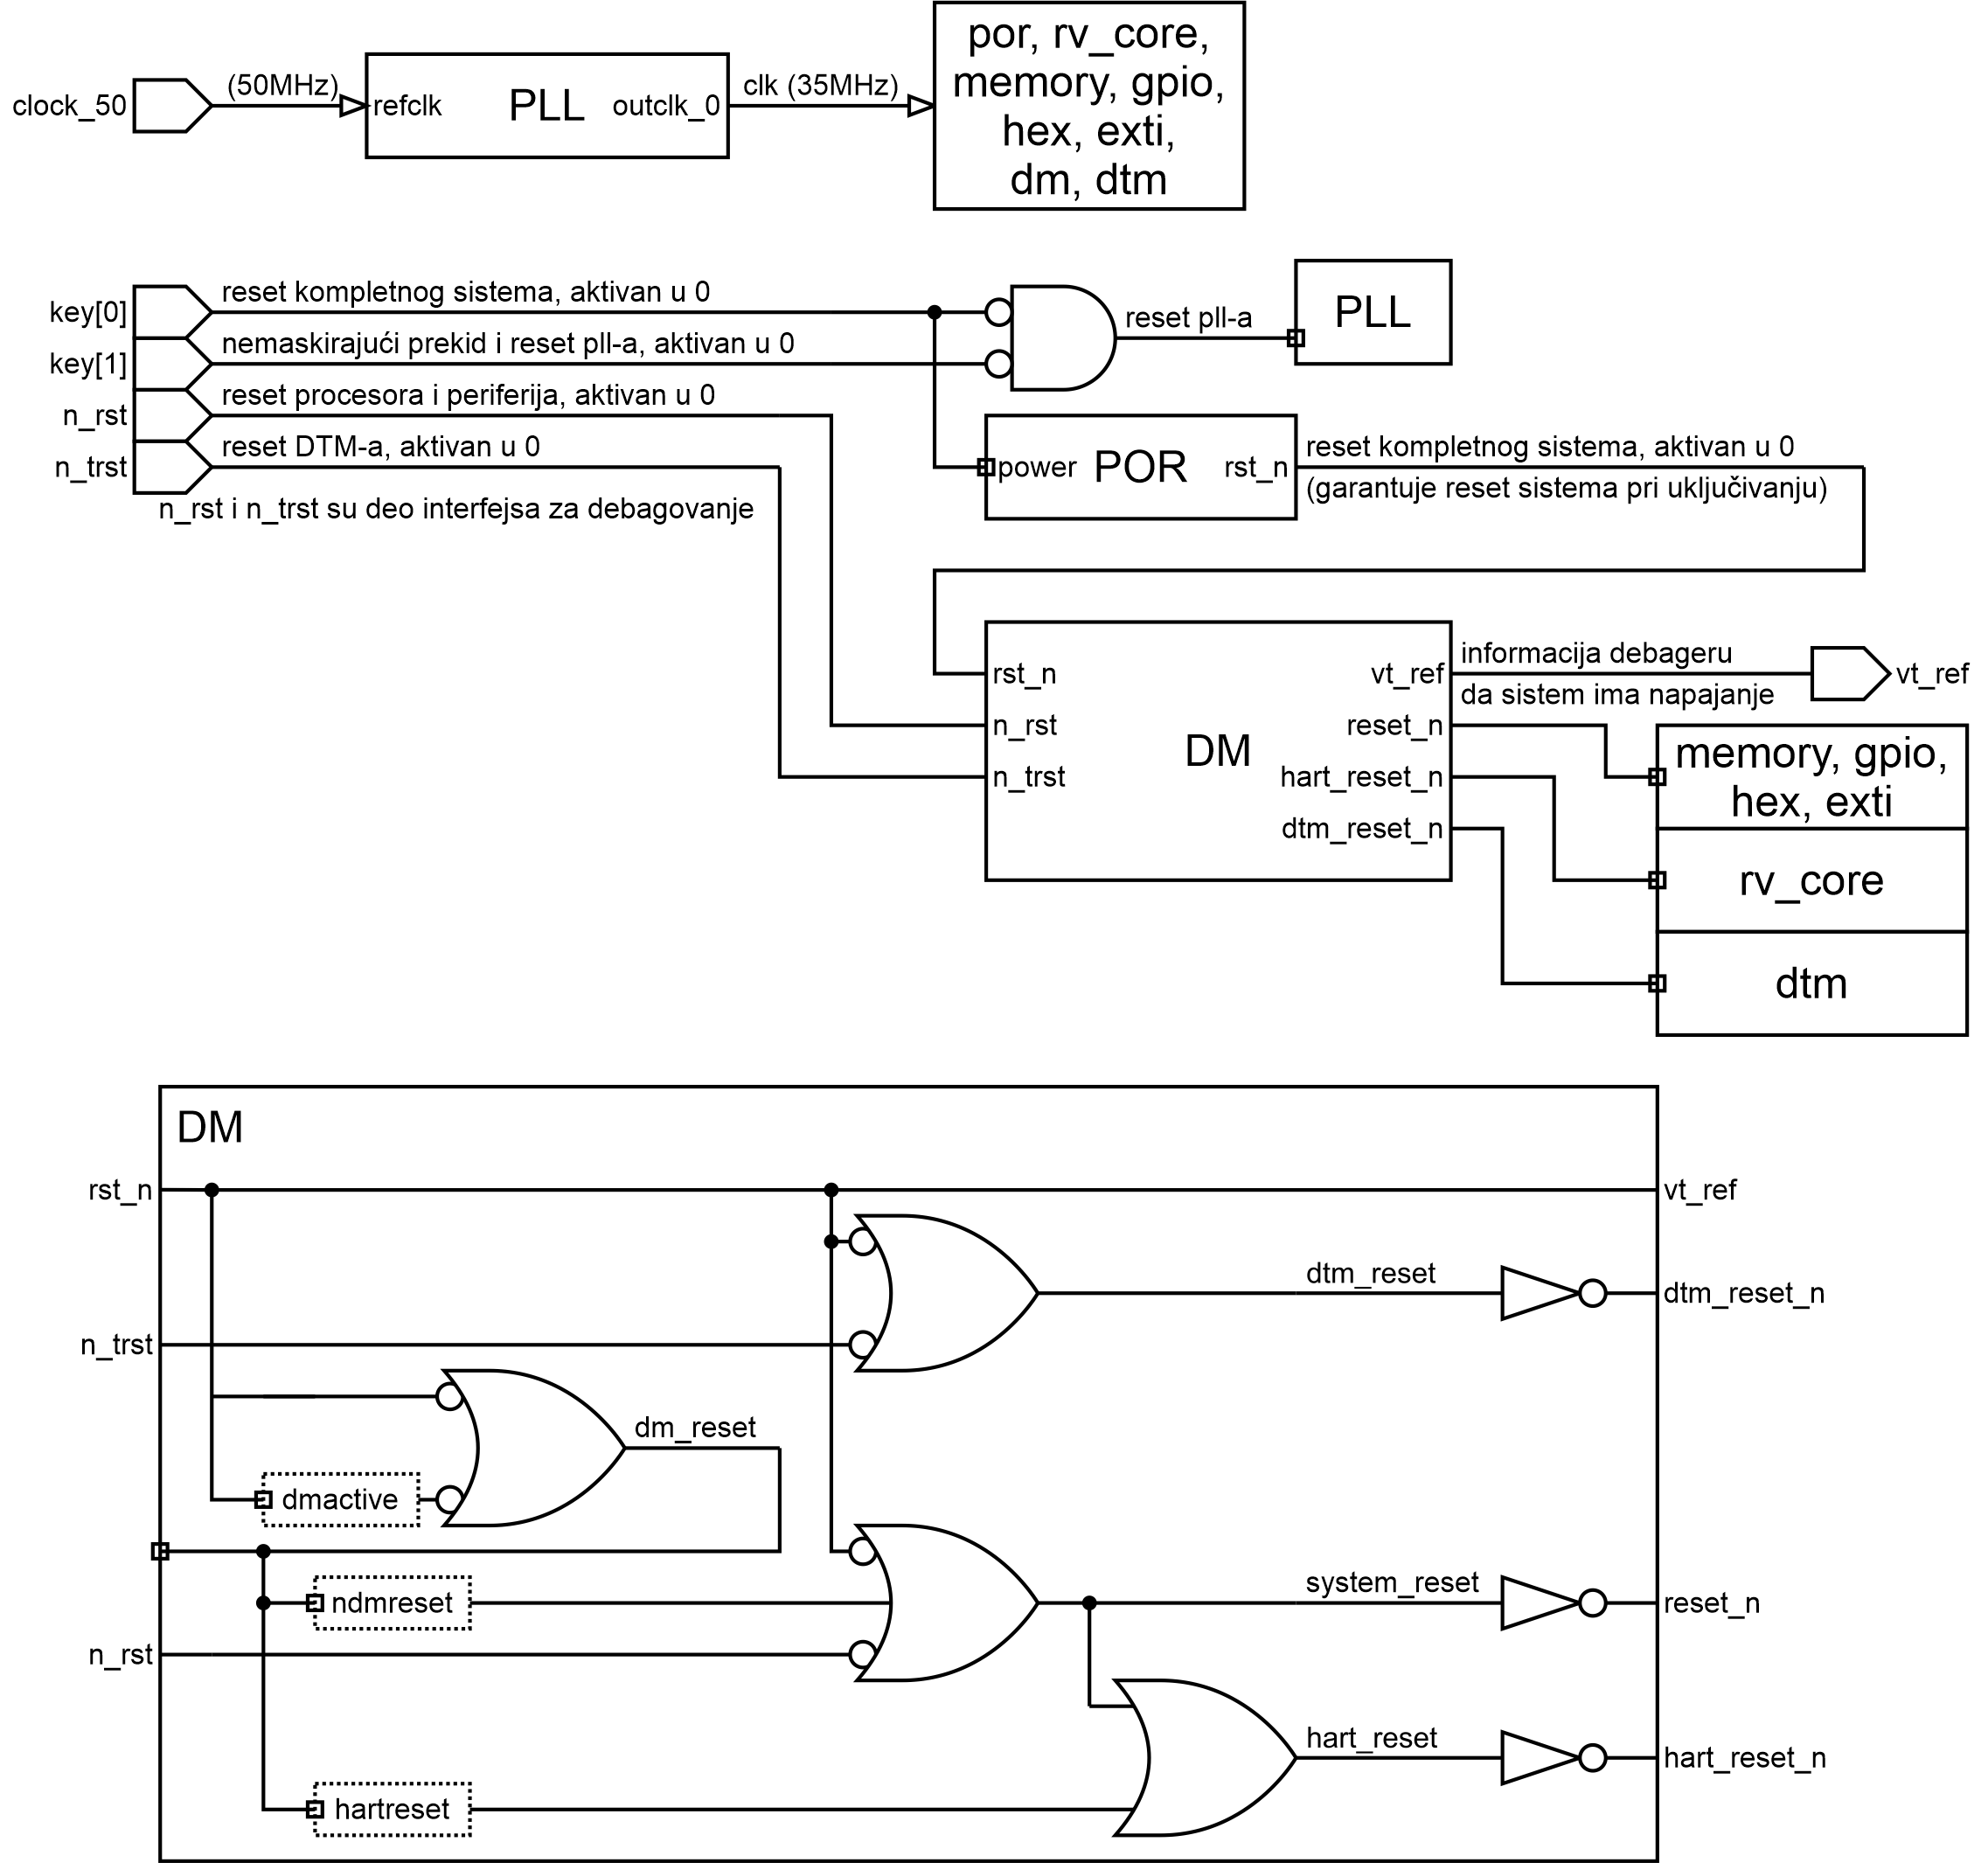
\includegraphics[width=\textwidth]{clkrst}
	\caption{Дијаграм сигнала такта и ресет сигнала}
	\label{fig:clkrst}
\end{figure}

\subsection{Сигнал такта}

Развојна плоча на себи има екстерни генератор сигнала такта који генерише такт фреквенције 50MHz. Екстерни сигнал такта улази на чип кроз пин \textbf{clock\_50} и иде директно у фазно закључану петљу која генерише сигнал такта фреквенције 35MHz, који се користи за остатак система. Како је фазно закључана петља део не конфигурабилног хардвера \фпга{} чипа, њен опис је генерисан помоћу чаробњака унутар \textit{Quartus} софтверског пакета. При генерисању фазно закључане петље коришћењем чаробњака, довољно је унети само фреквенцију улазног сигнала и жељену фреквенцију.  

\subsection{Ресет система}

Систем у потпуности користи синхроне ресет сигнале због ефикасније имплементације на \фпга{} чиповима. Постоји 6 ресет домена и то су:
\begin{itemize}
	\item Домен фазно закључане петље
	\item Домен ресета при покретању (енг. \textit{\acrfull{POR}})
	\item Домен \дм{}-a
	\item Домен \дтм{}-a
	\item Домен периферија и меморије
	\item Домен језгра
\end{itemize}

Фазно закључана петља се може ресетовати само уколико је комплетан остатак система такође под ресетом, што је могуће извршити активирањем захтева за немаскирајући прекид (\textbf{key[1]}) док је ресет комплетног система (\textbf{key[0]}) такође активан. Овакав неинтуитиван начин ресетовања је прихватљив јер се потреба за ресетовањем фазно закључане петље не очекује ван тестирања система.
Модул за ресет при покретању се као што му само име сугерише, аутоматски ресетује при покретању система (тј. након конфигурисања \фпга{} чипа) и када ресет комплетног система (\textbf{key[0]}) има активну вредност. Када се ресетује, модул за ресет при покретању задржава остатак система ресетованим подесиви број тактова.

Преостали домени су нешто комплекснији јер корисник има већу контролу над ресетовањем индивидуалних домена те њима управља \дм{}. Поред ова 4 домена, \дм{} управља још једним сигналом уско везаним за ресет система, a то је сигнал \textbf{vt\_ref} који даје до знања адаптеру за дебаговање да ли уређај има напајање, као и његов напон.
Сам \дм{} се ресетује при ресету комплетног система или уписом нуле у регистар \textbf{dmactive}\footnote{Упис у \textbf{dmactive} регистар је могућ и док је остатак \дм{}-а у ресету.}.
\дтм{} се ресетује комплетним ресетом система или активном вредношћу сигнала \textbf{n\_trst} који је део конектора за екстерно дебаговање.
Периферије и меморија\footnote{Треба навести да садржај меморије остаје непромењен.} се могу ресетовати комплетним ресетом система, сигналом \textbf{n\_rst} (такође део интерфејса за екстерно дебаговање) или битом \textbf{ndmreset} контролног регистра \дм{}-а.
Поред ресета периферија и меморије (који обухвата и само језгро), могуће је ресетовати и искључиво језгро коришћењем бита \textbf{hartreset} контролног регистра \дм{}-а.

\section{\textit{Arilla bus} магистрала}

\textit{Arilla bus} је магистрала за приступ меморији коришћена у ауторовим ранијим имплементацијама \рисцв{} процесора\cite{arilla}, а која је значајно редизајнирана и унапређена за потребе овог рада. У питању је синхрона магистрала са атомичним циклусима која може да обради једну операцију сваког такта. Кашњење података при упису је нула тактова а при читању је један такт. Приступи су на нивоу речи са избором бајтова који ће бити уписани.
Магистрала је конфигурабилна са произвољном ширином речи, адресе (наводи се ширина адресе са бајтовима као адресабилном јединицом јер је тако природније резоновати) и бајта. Активна вредност свих линија је 1.

\lstinputlisting[firstline = 4, lastline = 22,language=Verilog, caption=Линије које сачињавају \textit{Arilla bus} магистралу]{../src/system/arilla_bus_if.svh}

Постоје две линије за податке: \textbf{data\_ctp} (у смеру од језгра ка периферијама) и \textbf{data\_ptc} (у смеру од периферија ка језгру). Предност постојања две линије за податке је могућност извршавања операције уписа одмах након операције читања, што не би било могуће са једном линијом за податке због различитог кашњења података (видети такт 3 на слици \ref{fig:busop}). Како постоји само једна линија за адресу није могуће извршити и операцију читања и операцију писања у истом такту, ово је прихватљива одлука јер би у том случају меморија морала да буде вишепортна, што није толико често и компликује дизајн меморије. Линија \textbf{byte\_enable} представља маску бајтова који ће заправо бити уписани при операцији уписа (бајтови за које је одговарајући бит маске нула ће остати непромењени).

Магистрала има пет контролних линија. Линије \textbf{read} и \textbf{write} својом активном вредношћу означавају која операција ће бити извршена на магистрали. Понашање уколико обе линије имају активну вредност је \textbf{недефинисано}. Линија \textbf{hit} обавештава језгро да ли постоји меморија или периферија на тој адреси. У питању је комбинациони сигнал, концептуално имплементиран као ожичено или, међутим како \textit{Quartus} не подржава ожичено или које прелази границе модула, \textbf{hit} је у овом случају имплементиран експлицитним или колом.

Линија \textbf{inhibit} омогућава просту арбитрацију. Подизањем линије \textbf{inhibit} на активну вредност приоритетнији газда комбинационо забрањује мање приоритетном газди да извршава операције на магистрали. Приоритетнији газда онда у истом такту може извршити операцију на магистрали. Иако мање приоритетни газда не може да извршава операције на магистрали, то га не спречава да заврши већ започето читање података.

Линија \textbf{intercept} омогућава имплементацију уређаја који ослушкују магистралу. Када линија \textbf{intercept} има активну вредност, слуга коме тражена адреса припада неће поставити свој податак на одговарајућу линију, омогућавајући уређају који је поставио активну вредност \textbf{intercept} линије да постави податак на линију за податке. Одзив уређаја на промену ове линије је комбинациони. Постојање више уређаја који ослушкују се може реализовати уколико се линија \textbf{intercept} реализује као ожичено или, међутим уколико више слуга покушају да пресретну исти податак понашање је \textbf{недефинисано}. Ова функционалност може да омогући додавање тачака прекида у делове меморије који су намењени само за читање (енг. Read Only) пресретањем дохватања инструкција са тражене адресе, међутим тренутно није имплементиран ниједан уређај који користи ову линију, те је она ожичена на нулу. Разлог за то је непостојање подршке за овако нешто у спецификацији\cite{debug_spec}.

\begin{figure}[h!]
	\centering
	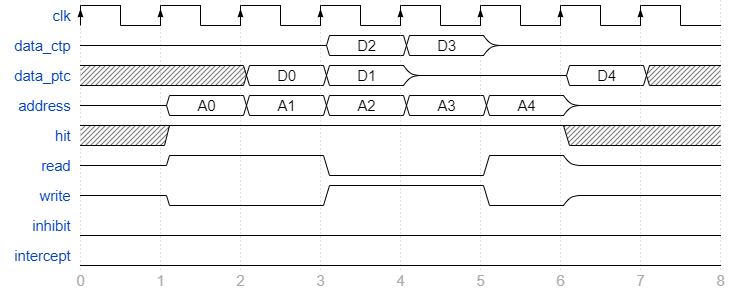
\includegraphics[width=\textwidth]{wavedrom}
	\caption{Дијаграм неколико операција \textit{Arilla bus} магистрале}
	\label{fig:busop}
\end{figure}

Слика \ref{fig:busop} приказује неколико узастопних циклуса на магистрали и на њој се може видети извршавање једне операције у једном такту, различита кашњења података за читање и упис и учешљавање операција на магистрали. Податак \textbf{D\textit{i}} представља податак у вези са адресом истог индекса.

\section{Меморија}

Имплементиран систем поседује 64КБ меморије за програм и податке. Меморија је имплементирана користећи интегрисане меморијске блокове \фпга{} чипа. Како меморијски блокови могу бити конфигурисани да имају карактеристике које захтева \textit{Arilla bus} магистрала, потребно је имплементирати само проверу адресе и руковање сигналима \textbf{data\_ptc} и \textbf{hit}.

\section{Периферије}

Развојна плоча \textit{DE10-Standard}\cite{de10} која је коришћена за имплементацију, поред самог \фпга{} чипа поседује и велики број периферија које су повезане на њега. Како би било могуће визуелно пратити стање извршавања програма ради поређења са стањем које приказује дебагер, одлучено је да се имплементира неколико простих периферија.

\subsection{\textit{\acrshort{GPIO}} периферија}

\textit{\acrfull{GPIO}} периферија је повезана на 10 прекидача и лед диода, као и 2 од 4 тастера. Ова периферија омогућава читање стања било којег од повезаних пинова и контролисање стања лед диода. Периферијом се управља кроз 3 регистра. \textit{\acrfull{DDR}} одређује да ли се неки пин користи као улазни или излазни, уколико је пин излазни, његов ниво је дефинисан одговарајућим битом \textit{\acrfull{DOR}} регистра, уколико је пин улазни, он се налази у стању високе импедансе како би екстерни сигнал могао да дефинише његов ниво. \textit{\acrfull{DIR}} регистар садржи информацију о напонском нивоу на сваком од пинова, то значи да је у теорији могуће детектовати уколико неки други уређај покушава да дефинише супротну вредност за неки од излазних пинова.

\lstinputlisting[language=C++, caption=Дефиниција регистара \textit{\acrshort{GPIO}} периферије]{../test/inc/gpio.h}

Периферија је конфигурабилна са подесивом базном адресом, бројем пинова (уколико је број пинова већи од ширине речи, потребан број речи за сваки од регистара ће бити аутоматски алоциран) и маском која спецификује пинове које се могу користити искључиво као улазни (њихови бити \textit{\acrshort{DDR}} регистра су ожичени на нулу\footnote{Исто важи и за неискоришћене бите у сва три регистра}).

\subsection{\textit{EXTI} периферија}

\textit{\acrfull{EXTI}} периферија је повезана на 10 прекидача и 2 од 4 тастера. Ова периферија омогућава генерисање захтева за прекид на узлазну и/или силазну ивицу било ког од повезаних пинова. Периферија поседује 5 регистара. \textit{\acrfull{IMR}} контролише који пинови могу да генеришу захтеве за прекиде, да би захтев за прекид био генерисан, неопходно је да одговарајући бити буду постављени и у \textit{\acrshort{IMR}} и у \textit{\acrshort{IPR}} регистру. \textit{\acrfull{IPR}} садржи информацију о томе са којих пинова су пристигли захтеви за прекиде, бит овог регистра ће аутоматски бити постављен уколико се на одговарајућој линији детектује ивица и \textit{\acrshort{RER}} и \textit{\acrshort{FER}} регистри су подешени да ту ивицу детектују. Одговарајући бит \textit{\acrshort{IPR}} регистра се брише уписивањем јединице у њега. \textit{\acrfull{ISR}} омогућава софтверу да ручно генерише прекид на некој линији уписивањем јединице у одговарајући бит. Регистри  \textit{\acrfull{RER}} и \textit{\acrfull{FER}} контролишу на које ивице (узлазну, силазну или обе) ће бити генерисан захтев за прекид.

\lstinputlisting[firstline = 6, lastline = 17,language=C++, caption=Дефиниција регистара \textit{\acrshort{EXTI}} периферије]{../test/inc/exti.h}

Периферија је конфигурабилна са подесивом базном адресом и бројем пинова.

\subsection{\textit{HEX} периферија}

\textit{\textit{HEX}} периферија контролише 6 седмосегментних дисплеја који постоје на развојној плочи.
Периферија поседује три мода операције који се бирају уписом одговарајуће вредности у \textit{MODE} регистар.
У \textit{DEC} или \textit{HEX} моду дисплеји приказују вредност одговарајућег броја најнижих бита \textit{DATA} регистра у одговарајућем бројевном систему, док се у \textit{MAN} моду за сваки дисплеј алоцира по 8 бита где 7 најнижих бита директно контролише индивидуалне сегменте дисплеја. 

\lstinputlisting[firstline = 6, lastline = 17,language=C++, caption=Дефиниција регистара \textit{HEX} периферије]{../test/inc/hex.h}

Периферија је конфигурабилна са подесивом базном адресом и бројем дисплеја, као што се може видети, уколико је потребно периферија алоцира више меморијских речи за \textit{DATA} регистар.

\subsection{Интерфејс за меморијски мапиране регистре}

Све периферије које поседују меморијски мапиране регистре користе \textbf{periph\_mem\_interface} компоненту која пружа једноставан интерфејс за имплементацију меморијски мапираних регистара. Компонента прима базну адресу и величину меморијски мапираног региона у речима (величина мора бити  степен броја 2, одговорност је на периферији која користи ову компоненту да своје регистре прошири ожиченим нулама до потребног броја речи), све остале параметре меморијске магистрале компонента детектује аутоматски. Интерфејс према периферији која користи ову компоненту се састоји од три линије \textbf{data\_periph\_in}, \textbf{data\_periph\_out}, \textbf{data\_periph\_write}. Линија \textbf{data\_periph\_in} је величине \textit{Ширина речи * Број речи} и представља податке које периферија жели да учини доступним. Линија \textbf{data\_periph\_out} (ширине меморијске речи) представља податке које језгро жели да упише на неку адресу меморијски мапираног региона, излаз ове линије имплементира маску бајтова за упис те није потребно да периферија имплементира ту функционалност. Линија \textbf{data\_periph\_write} поседује по један бит за сваку меморијску реч меморијски мапираног региона, одговарајући бит ове линије има активну вредност када језгро врши упис у ту меморијску реч.\newpage

\lstinputlisting[firstline = 3, lastline = 36,language=Verilog, caption=Портови \textbf{periph\_mem\_interface} компоненте]{../src/components/periph_mem_interface.sv}